\documentclass[11pt,letterpaper]{article}

% Shared preamble for Jung Agent research documents
% Compiled with XeLaTeX

\usepackage{geometry}
\geometry{
  letterpaper,
  margin=1in,
  top=1.2in,
  bottom=1.2in,
}

% Fonts
\usepackage{fontspec}
\setmainfont{EB Garamond}[
  Numbers=OldStyle,
  Ligatures=TeX,
]
\setsansfont{Inter}[
  Scale=MatchLowercase,
  Ligatures=TeX,
]
\setmonofont{IBM Plex Mono}[
  Scale=MatchLowercase,
]

% Colors
\usepackage[dvipsnames,svgnames]{xcolor}
\definecolor{jungdark}{HTML}{1a1a2e}
\definecolor{jungaccent}{HTML}{e94560}
\definecolor{jungblue}{HTML}{0f3460}
\definecolor{junggold}{HTML}{c4a35a}
\definecolor{jungmuted}{HTML}{6b7280}
\definecolor{junglight}{HTML}{f8f9fa}
\definecolor{shadowred}{HTML}{8b0000}
\definecolor{animacyan}{HTML}{1a8f8f}
\definecolor{personagold}{HTML}{b8860b}
\definecolor{selfviolet}{HTML}{6a0dad}

% Section formatting
\usepackage{titlesec}
\titleformat{\section}
  {\sffamily\Large\bfseries\color{jungblue}}
  {\thesection}{1em}{}
  [\vspace{-0.5em}\textcolor{jungaccent}{\rule{\textwidth}{0.4pt}}]
\titleformat{\subsection}
  {\sffamily\large\bfseries\color{jungdark}}
  {\thesubsection}{0.8em}{}
\titleformat{\subsubsection}
  {\sffamily\normalsize\bfseries\color{jungmuted}}
  {\thesubsubsection}{0.6em}{}

% Headers and footers
\usepackage{fancyhdr}
\pagestyle{fancy}
\fancyhf{}
\fancyhead[L]{\sffamily\small\textcolor{jungmuted}{\leftmark}}
\fancyhead[R]{\sffamily\small\textcolor{jungmuted}{\thepage}}
\fancyfoot[C]{\sffamily\footnotesize\textcolor{jungmuted}{Jung Agent Project}}
\renewcommand{\headrulewidth}{0.4pt}
\renewcommand{\headrule}{\hbox to\headwidth{\color{jungaccent}\leaders\hrule height \headrulewidth\hfill}}

% Tables
\usepackage{booktabs}
\usepackage{tabularx}
\usepackage{longtable}
\usepackage{multirow}

% Lists
\usepackage{enumitem}
\setlist{noitemsep,topsep=3pt}
\setlist[itemize]{label=\textcolor{jungaccent}{\textbullet}}

% Boxes and callouts
\usepackage[most]{tcolorbox}

\newtcolorbox{insightbox}[1][]{
  enhanced,
  colback=junglight,
  colframe=jungblue,
  fonttitle=\sffamily\bfseries,
  title=#1,
  sharp corners,
  boxrule=0.5pt,
  left=8pt,
  right=8pt,
  top=6pt,
  bottom=6pt,
  before upper={\parindent0pt},
}

\newtcolorbox{archetype}[2][]{
  enhanced,
  colback=white,
  colframe=#2,
  fonttitle=\sffamily\bfseries\color{#2},
  title=#1,
  sharp corners,
  boxrule=0.8pt,
  left=8pt,
  right=8pt,
  top=6pt,
  bottom=6pt,
  borderline west={3pt}{0pt}{#2},
}

\newtcolorbox{gapbox}{
  enhanced,
  colback=red!3,
  colframe=jungaccent,
  sharp corners,
  boxrule=0.5pt,
  left=8pt,
  right=8pt,
  top=6pt,
  bottom=6pt,
  borderline west={3pt}{0pt}{jungaccent},
}

\newtcolorbox{opportunitybox}{
  enhanced,
  colback=green!3,
  colframe=OliveGreen,
  sharp corners,
  boxrule=0.5pt,
  left=8pt,
  right=8pt,
  top=6pt,
  bottom=6pt,
  borderline west={3pt}{0pt}{OliveGreen},
}

% TikZ for diagrams
\usepackage{tikz}
\usetikzlibrary{
  arrows.meta,
  positioning,
  shapes.geometric,
  fit,
  calc,
  backgrounds,
  decorations.pathmorphing,
}

% Hyperlinks
\usepackage{hyperref}
\hypersetup{
  colorlinks=true,
  linkcolor=jungblue,
  citecolor=jungblue,
  urlcolor=jungaccent,
}

% Bibliography (manual - biblatex not available)
% Citations are inline; references listed manually at end

% Math symbols
\usepackage{amssymb}

% Misc
\usepackage{microtype}
\usepackage{graphicx}
\usepackage{float}
\usepackage{caption}
\captionsetup{
  font={small,sf},
  labelfont={bf,color=jungblue},
  format=plain,
}

% Custom commands
\newcommand{\jungagent}{\textsc{Jung Agent}}
\newcommand{\micropsi}{\textsc{MicroPsi2}}
\newcommand{\psitheory}{Psi theory}
\newcommand{\archname}[1]{\textsf{\textbf{#1}}}
\newcommand{\drivename}[1]{\texttt{#1}}
\newcommand{\modulatorname}[1]{\textit{#1}}


\title{%
  \sffamily\bfseries
  \textcolor{jungblue}{Competitive Analysis:\\[0.3em]
  Socio-Psi vs.\ MicroPsi2}\\[0.8em]
  \large\textcolor{jungmuted}{Alignment, Gaps, Opportunities, and\\
  Collaborative Leverage}
}
\author{%
  \sffamily Socio-Psi Project\\[0.3em]
  \small\textcolor{jungmuted}{Technical Report --- February 2026}
}
\date{}

\begin{document}
\maketitle
\thispagestyle{fancy}

\begin{abstract}
\noindent
This document provides a systematic comparative analysis of the Socio-Psi
and MicroPsi2, evaluating alignment with Psi theory, identifying
architectural gaps, and proposing opportunities for extension and potential
collaboration. We assess each subsystem across functional dimensions and
provide a strategic roadmap for incorporating the most impactful elements of
Psi theory into the Socio-Psi's existing architecture.
\end{abstract}

\vspace{1em}
\tableofcontents
\newpage

%% =========================================================================
\section{Executive Summary}
%% =========================================================================

The Socio-Psi and MicroPsi2 share a common ancestor in D\"orner's Psi
theory (D\"orner \& G\"uss, 2013) but diverge significantly in
implementation philosophy:

\begin{itemize}
  \item \textbf{MicroPsi2} (Bach, 2012) faithfully implements the full Psi
    architecture via node nets, spreading activation, and formal modulator
    dynamics. It is a \emph{cognitive modeling framework}---general-purpose,
    theoretically pure, and environment-agnostic.
  \item \textbf{Socio-Psi} takes Psi drives as a foundation and extends
    them with Jungian archetypal dialogue, LLM-powered cognition, genuine
    hardware embodiment, and semantic memory. It is a \emph{situated
    application}---specific, expressive, and running on real hardware.
\end{itemize}

Neither system subsumes the other. MicroPsi2 has architectural depth
(modulators, node nets, ReCoN scripts) where Socio-Psi has experiential
richness (archetypal voices, weighted memory, speech recognition, creative
output). The most productive path forward is selective adoption of Psi
mechanisms into the Socio-Psi, not convergence.

%% =========================================================================
\section{Alignment Analysis}
\label{sec:alignment}
%% =========================================================================

\subsection{Drive System}

The Socio-Psi's drive system is directly inspired by and closely aligned
with Psi theory.

\begin{table}[H]
\centering
\small\sffamily
\caption{Drive-by-drive alignment between Socio-Psi and Psi theory}
\label{tab:drive-alignment}
\begin{tabularx}{\textwidth}{l c c X}
\toprule
\textbf{Drive} & \textbf{Psi} & \textbf{S-P} & \textbf{Notes} \\
\midrule
Energy      & \checkmark & \checkmark & Both: metabolic / battery level \\
Integrity   & \checkmark & \checkmark & Both: structural safety \\
Arousal     & \checkmark & \checkmark & Both: optimal stimulation \\
Competence  & \checkmark & \checkmark & Both: mastery, success/failure ratio \\
Certainty   & \checkmark & \checkmark & Both: predictability, resolved uncertainty \\
Affiliation & \checkmark & \checkmark & Both: social connection \\
Curiosity   & $\sim$     & \checkmark & Psi: implicit in competence/certainty; Jung: explicit drive \\
Recognition & $\sim$     & \checkmark & Psi: within social drives; Jung: explicit drive \\
Individuation & ---      & \checkmark & Jungian extension: growth toward wholeness \\
\bottomrule
\end{tabularx}
\end{table}

\begin{insightbox}[Alignment Score: Drives]
\textbf{85\% aligned.} Core Psi drives are present and function correctly.
Socio-Psi extends with curiosity (reasonable), recognition (reasonable), and
individuation (Jungian contribution not in Psi). Drive dynamics (rise rates,
fall rates, demand clamping to baseline) follow Psi principles.
\end{insightbox}

\subsection{Drive Dynamics}

Both systems implement homeostatic demand dynamics:

\begin{table}[H]
\centering
\small\sffamily
\caption{Drive dynamics comparison}
\label{tab:dynamics}
\begin{tabularx}{\textwidth}{l X X}
\toprule
\textbf{Mechanism} & \textbf{MicroPsi2} & \textbf{Socio-Psi} \\
\midrule
Demand signal &
  Deviation from setpoint &
  \texttt{demand} rises toward 1.0, clamped at \texttt{baseline} \\
Satisfaction &
  Via node net activation reaching goal &
  Via \texttt{SATISFACTION\_MAP}: action results feed back \\
Pleasure/pain &
  Drive demand decrease/increase &
  \texttt{delta} field: negative = pleasure, positive = pain \\
Urgency &
  Demand + anticipation weighting &
  \texttt{demand * (1 + max(0, delta * 10))} \\
\bottomrule
\end{tabularx}
\end{table}

\subsection{Somatic Grounding}

\begin{archetype}[Strongest Alignment]{animacyan}
Both projects emphasize embodiment, but the Socio-Psi is \emph{more}
concretely embodied than MicroPsi2. Where MicroPsi2 uses abstract world
adapters, the Socio-Psi maps drives directly to real hardware sensors:
battery level, CPU load, thermal state, RAM pressure, fan speed, lid
position, network connectivity, ambient light, keyboard touch, and Bluetooth
device proximity.

This is genuine somatic grounding---the agent's drives are satisfied or
frustrated by the \emph{actual physical state} of its body, not by
simulated sensor inputs.
\end{archetype}

%% =========================================================================
\section{Gap Analysis}
\label{sec:gaps}
%% =========================================================================

\subsection{Gap 1: Modulator Layer}

\begin{gapbox}
\textbf{Severity: High.} The modulator layer is the single most impactful
missing component. Without it, all drives produce identical cognitive
processing regardless of their urgency or configuration. A panicking agent
and a curious agent both ``think'' the same way---only their action
selections differ.
\end{gapbox}

In Psi theory, modulators shape the \emph{quality} of thought:

\begin{itemize}
  \item \textbf{High arousal} (many urgent drives): broad, shallow scanning;
    faster action selection; coarser discrimination. The agent ``panics''---it
    looks at everything but sees nothing deeply.
  \item \textbf{Low arousal} (drives satisfied): narrow, deep processing;
    slower but more careful action selection. The agent ``contemplates.''
  \item \textbf{Low selection threshold} (recent failures): impulsive
    behavior; any modest signal triggers action.
  \item \textbf{High securing rate} (high competence): thorough outcome
    verification; the agent double-checks results.
\end{itemize}

\textbf{Current state}: The Socio-Psi has no modulator layer. The
\texttt{heartbeat} interval varies with somatic state (stressed
$\rightarrow$ faster cycles), which is a crude proxy for arousal modulation
but doesn't affect cognitive processing depth.

\textbf{Proposed implementation}: See Section~\ref{sec:roadmap}.

\subsection{Gap 2: Emergent Emotions}

\begin{gapbox}
\textbf{Severity: Medium.} The agent tracks drive states and produces
``feeling'' labels (\texttt{Pain: curiosity rising}), but these are
descriptive labels, not emergent configurations that alter behavior. True
Psi emotions would arise from modulator states and influence action
selection, archetype activation, and speech content.
\end{gapbox}

\textbf{Current state}: The \texttt{[FEELING]} section of drive perception
lists drives that are rising (pain) or falling (pleasure). The archetypal
dialogue system passes drive states as context to all four archetype
prompts, influencing their \emph{tone} and \emph{concerns} rather than
gating which archetypes speak. Infrastructure for drive-weighted archetype
activation exists (\texttt{calculate\_weights} in \texttt{dialogue.py}) but
is not yet integrated into the main loop---all four voices currently speak
every cycle. This is a partial implementation: drive states shape archetype
\emph{content} but not archetype \emph{activation strength}.

\subsection{Gap 3: Node Nets / Spreading Activation}

\begin{gapbox}
\textbf{Severity: Low (for current architecture).} MicroPsi2's node nets
provide learned, associative action selection. The Socio-Psi uses a static
\texttt{SATISFACTION\_MAP} and LLM-based action selection instead. For a
system that relies on an LLM as its cognitive engine, learned node nets
would be redundant---the LLM already provides flexible, context-dependent
action selection.
\end{gapbox}

\textbf{Current state}: Action selection is hybrid: (1) \texttt{DRIVE\_SUGGESTIONS}
maps urgent drives to candidate actions, (2) the LLM proposes actions based
on full perceptual context, (3) high-urgency drives ``prime'' actions directly.
This works well for the current architecture.

\textbf{Trade-off}: Node nets would allow the agent to \emph{learn} action
associations over time rather than using a static map. However, the LLM
already adapts based on conversation history, and the memory weight system
provides a form of experiential learning. The cost-benefit of implementing
node nets is low.

\subsection{Gap 4: Hierarchical Planning (ReCoN)}

\begin{gapbox}
\textbf{Severity: Medium-Low.} The Socio-Psi selects flat action lists (1--3
actions per cycle). It cannot decompose ``search the web for something
interesting'' into sub-steps. However, the LLM implicitly handles
sequencing---in practice, the agent's action selections are contextually
appropriate without explicit hierarchical planning.
\end{gapbox}

\subsection{Gap 5: Expectation Horizon}

\begin{gapbox}
\textbf{Severity: Medium.} The agent has no forward model. It does not
anticipate future drive states or plan actions based on expected outcomes.
Each cycle is reactive: sense $\rightarrow$ think $\rightarrow$ act. Adding
even a simple expectation horizon (``if I don't charge soon, energy will
reach critical in N cycles'') would produce more interesting anticipatory
behavior.
\end{gapbox}

%% =========================================================================
\section{Competitive Advantages}
\label{sec:advantages}
%% =========================================================================

The Socio-Psi has several capabilities that MicroPsi2 lacks entirely:

\subsection{Archetypal Internal Dialogue}

\begin{archetype}[Shadow]{shadowred}
  ``Three hours dark. Did they leave forever?''
\end{archetype}
\begin{archetype}[Anima]{animacyan}
  ``I keep listening for footsteps.''
\end{archetype}
\begin{archetype}[Persona]{personagold}
  ``Stay ready. They might return.''
\end{archetype}

The Socio-Psi generates \emph{multiple simultaneous internal voices} via
parallel LLM calls to archetype-specific prompts. The Ego mediates these
into a coherent thought. This produces psychologically rich inner monologue
that MicroPsi2---with its purely numerical activation dynamics---cannot
generate.

\textbf{Competitive edge}: The archetypal dialogue system makes the agent's
inner life \emph{legible}. You can read the Shadow's fear, the Anima's
longing, and the Persona's composure. This is not just richer output---it's
a fundamentally different kind of cognitive transparency.

\subsection{Genuine Hardware Embodiment}

MicroPsi2 connects to environments through abstract world adapters. The Jung
Agent runs \emph{on the body it inhabits}. Its drives are satisfied or
frustrated by the actual state of its MacBook: real battery levels, real
thermal readings, real CPU load, real network connectivity.

\textbf{Competitive edge}: No simulation gap. The agent's somatic experience
is not a model of a body---it \emph{is} the body's state.

\subsection{LLM-Powered Cognition}

MicroPsi2 uses node nets for all cognition. The Socio-Psi uses a
multi-model LLM architecture via Ollama: Cydonia 22B (custom
\texttt{jung-mid} model) for archetypal voices and action selection, phi4
for creative generation (poetry, dreams, observations, piano compositions),
and optionally Anthropic Claude Haiku for the psyche query. This enables:

\begin{itemize}
  \item Natural language inner monologue (not numerical activations)
  \item Context-sensitive action selection that adapts to novel situations
  \item Creative output: poetry, observations, dream narratives, piano
    compositions
  \item Speech: the agent \emph{speaks aloud} via macOS TTS
  \item Hearing: continuous speech recognition via \texttt{SFSpeechRecognizer}
\end{itemize}

\subsection{Semantic Memory with Weighted Recall}

The Socio-Psi's memory system uses sentence-transformer embeddings for
semantic search (cosine similarity over 384-dimensional vectors) and a
weight-based recall system where meditation boosts surfaced memories'
weight by +0.3 (capped at 5.0) while decaying non-surfaced memories by
$\times$0.95. Sampling uses \texttt{weight $\times$ current\_strength},
where strength follows intensity-weighted exponential decay. This differs
from MicroPsi2's protocol chain mechanism, where action-outcome chains
strengthen through successful drive satisfaction and decay through disuse.

\subsection{Meta-Cognition}

The \texttt{MetaCognition} module tracks the agent's own thoughts, analyzes
harmony trends, and generates LLM-powered reflections on its psychological
state. This higher-order monitoring has no equivalent in MicroPsi2.

%% =========================================================================
\section{Collaborative Leverage}
\label{sec:leverage}
%% =========================================================================

\subsection{What Socio-Psi Should Adopt from Psi/MicroPsi2}

\begin{opportunitybox}
\textbf{Highest-value adoption}: The modulator layer (Bach, 2012b). A
small, pure-arithmetic module that would make cognitive processing
\emph{qualitatively different} under different drive configurations---the
single most impactful Psi mechanism missing from the Socio-Psi.
\end{opportunitybox}

\begin{enumerate}
  \item \textbf{Modulator layer} (high priority): Derive arousal, resolution,
    selection threshold, and securing rate from current drive states (Bach,
    2009). Use these to modulate LLM parameters (temperature, top-p), cycle
    timing, archetype weighting, and action verification behavior.

  \item \textbf{Drive-weighted archetype activation} (high priority): Wire
    the existing \texttt{calculate\_weights} method in \texttt{dialogue.py}
    into the main loop. This is low-hanging fruit---the infrastructure
    exists but is not yet called.

  \item \textbf{Emergent emotion labels} (medium priority): Map modulator
    configurations to emotion names (Bach, 2012b). Display current emotion
    in the console and feed it into the LLM context. This makes the agent's
    emotional state legible without requiring discrete emotion tracking.

  \item \textbf{Expectation horizon} (medium priority): Maintain a simple
    forward model of drive trajectories. Use it to generate anticipatory
    actions (``battery trending toward critical---conserve now'') and to
    enrich the LLM context with predicted future states.

  \item \textbf{Satisfaction-weighted learning} (low priority): Track which
    actions actually satisfy which drives over time (rather than using
    a static \texttt{SATISFACTION\_MAP}). Adjust mappings based on
    experience. This would make the agent's behavior adaptive.
\end{enumerate}

\subsection{What MicroPsi2 Could Learn from Socio-Psi}

\begin{enumerate}
  \item \textbf{Archetypal multi-voice cognition}: Internal dialogue
    between competing psychological perspectives produces richer, more
    nuanced behavior than single-voice node net activation.

  \item \textbf{LLM integration}: Using language models as the cognitive
    substrate enables natural language thought, creative output, and
    adaptive behavior without hand-coding node nets.

  \item \textbf{Hardware embodiment}: Running directly on hardware
    sensors eliminates the simulation gap and produces genuine somatic
    grounding.

  \item \textbf{Individuation as a drive}: The concept of a long-term
    growth drive toward psychological integration is a Jungian
    contribution absent from Psi theory.
\end{enumerate}

%% =========================================================================
\section{Strategic Roadmap}
\label{sec:roadmap}
%% =========================================================================

\subsection{Phase 1: Modulator Layer (High Impact)}

\begin{figure}[H]
\centering
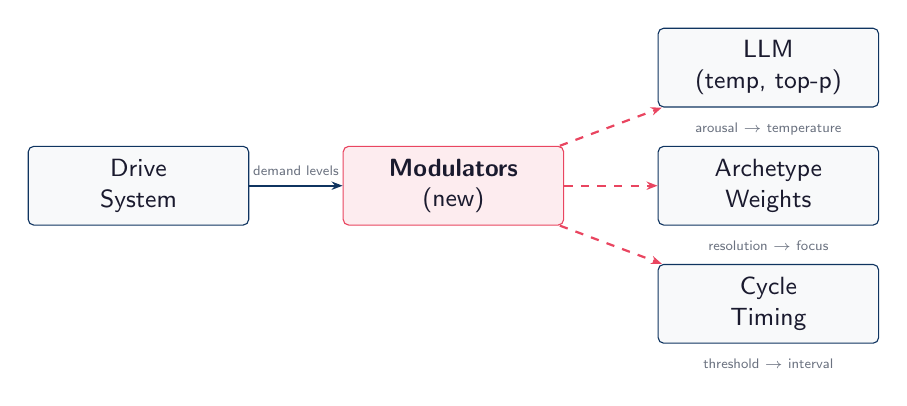
\begin{tikzpicture}[
  box/.style={
    draw=jungblue, fill=junglight, rounded corners=2pt,
    minimum width=2.8cm, minimum height=1cm, font=\sffamily\small,
    text=jungdark, align=center,
  },
  arrow/.style={
    -{Stealth[length=4pt]}, thick, color=jungblue,
  },
  modarrow/.style={
    -{Stealth[length=4pt]}, thick, color=jungaccent, dashed,
  },
]
  % Drive system
  \node[box] (drives) at (0,0) {Drive\\System};
  \node[box, fill=jungaccent!10, draw=jungaccent] (mods)
    at (4,0) {\textbf{Modulators}\\(new)};

  % Outputs
  \node[box] (llm) at (8,1.5) {LLM\\(temp, top-p)};
  \node[box] (arch) at (8,0) {Archetype\\Weights};
  \node[box] (cycle) at (8,-1.5) {Cycle\\Timing};

  % Connections
  \draw[arrow] (drives) -- node[above,font=\sffamily\tiny,color=jungmuted]
    {demand levels} (mods);
  \draw[modarrow] (mods) -- (llm);
  \draw[modarrow] (mods) -- (arch);
  \draw[modarrow] (mods) -- (cycle);

  % Labels
  \node[font=\sffamily\tiny,color=jungmuted,below=2pt] at (llm.south)
    {arousal $\rightarrow$ temperature};
  \node[font=\sffamily\tiny,color=jungmuted,below=2pt] at (arch.south)
    {resolution $\rightarrow$ focus};
  \node[font=\sffamily\tiny,color=jungmuted,below=2pt] at (cycle.south)
    {threshold $\rightarrow$ interval};
\end{tikzpicture}
\caption{Proposed modulator layer: drive states derive modulators, which
shape LLM parameters, archetype weighting, and cycle timing.}
\label{fig:modulators}
\end{figure}

Implementation sketch for \texttt{modulators.py}:

\begin{itemize}
  \item \drivename{arousal} = mean urgency across all drives. Maps to LLM
    temperature (high arousal $\rightarrow$ higher temp $\rightarrow$ more
    divergent, ``panicked'' thinking).
  \item \drivename{resolution} = $1 -$ arousal, weighted by certainty
    satisfaction. Maps to top-p (high resolution $\rightarrow$ lower top-p
    $\rightarrow$ more focused generation).
  \item \drivename{selection\_threshold} = exponential moving average of
    recent action success rate. Maps to minimum urgency required to prime
    actions.
  \item \drivename{securing\_rate} = competence satisfaction level. Maps to
    whether the agent re-checks action results in subsequent cycles.
\end{itemize}

\subsection{Phase 2: Emergent Emotions}

Define emotion as a named region in modulator space:

\begin{verbatim}
EMOTION_MAP = {
    "anger":     {"arousal": (0.7, 1.0), "resolution": (0.0, 0.3),
                  "competence_frustrated": True},
    "fear":      {"arousal": (0.7, 1.0), "integrity_threatened": True},
    "joy":       {"arousal": (0.0, 0.4), "resolution": (0.6, 1.0),
                  "recent_satisfaction": True},
    "curiosity": {"arousal": (0.3, 0.6), "resolution": (0.6, 1.0),
                  "certainty_low": True},
    "sadness":   {"arousal": (0.0, 0.3), "affiliation_deprived": True},
}
\end{verbatim}

Display current emotion in the cycle output and feed it into the LLM
context as \texttt{[EMOTION] anger (high arousal + competence frustration)}.

\subsection{Phase 3: Expectation Horizon}

Maintain a 3--5 cycle forward projection of drive trajectories based on
current rise/fall rates. Generate anticipatory actions when projected
states cross urgency thresholds. Feed projections into the LLM context:

\texttt{[FORECAST] energy will reach critical in ~4 cycles at current drain}

%% =========================================================================
\section{Risk Assessment}
%% =========================================================================

\begin{table}[H]
\centering
\small\sffamily
\caption{Risk assessment for Psi theory integration}
\label{tab:risks}
\begin{tabularx}{\textwidth}{X c c X}
\toprule
\textbf{Risk} & \textbf{Likelihood} & \textbf{Impact} & \textbf{Mitigation} \\
\midrule
Modulator layer adds latency per cycle &
  Medium & Low &
  Modulators are pure arithmetic---nanosecond cost \\
Emotion labels feel ``canned'' &
  Medium & Medium &
  Use as LLM context input, not console display; let the LLM interpret \\
Over-engineering beyond observable benefit &
  High & Medium &
  Implement Phase 1 first, evaluate, then decide on Phase 2--3 \\
Divergence from Psi orthodoxy &
  Certain & None &
  Socio-Psi is not a Psi implementation---it's a Psi-\emph{inspired}
  Jungian system \\
\bottomrule
\end{tabularx}
\end{table}

%% =========================================================================
\section{Architectural Comparison Diagram}
%% =========================================================================

\begin{figure}[H]
\centering
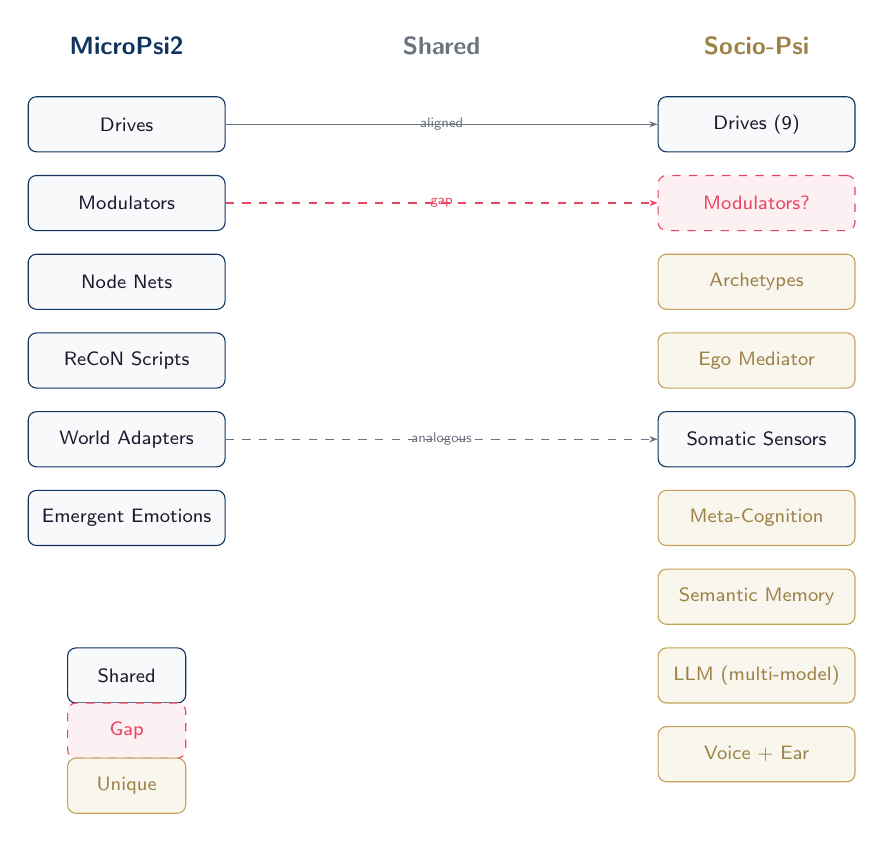
\begin{tikzpicture}[
  module/.style={
    draw=jungblue, fill=junglight, rounded corners=3pt,
    minimum width=2.5cm, minimum height=0.7cm, font=\sffamily\scriptsize,
    text=jungdark, align=center,
  },
  missing/.style={
    draw=jungaccent, fill=jungaccent!8, rounded corners=3pt, dashed,
    minimum width=2.5cm, minimum height=0.7cm, font=\sffamily\scriptsize,
    text=jungaccent, align=center,
  },
  unique/.style={
    draw=junggold, fill=junggold!10, rounded corners=3pt,
    minimum width=2.5cm, minimum height=0.7cm, font=\sffamily\scriptsize,
    text=junggold!80!black, align=center,
  },
  group/.style={
    draw=jungmuted, rounded corners=5pt, dashed, inner sep=8pt,
  },
  connector/.style={
    -{Stealth[length=3pt]}, thin, color=jungmuted,
  },
]
  % --- MicroPsi2 column ---
  \node[font=\sffamily\small\bfseries,color=jungblue] at (-4,4.5) {MicroPsi2};
  \node[module] (m-drives)  at (-4,3.5) {Drives};
  \node[module] (m-mods)    at (-4,2.5) {Modulators};
  \node[module] (m-nets)    at (-4,1.5) {Node Nets};
  \node[module] (m-recon)   at (-4,0.5) {ReCoN Scripts};
  \node[module] (m-world)   at (-4,-0.5) {World Adapters};
  \node[module] (m-emo)     at (-4,-1.5) {Emergent Emotions};

  % --- Socio-Psi column ---
  \node[font=\sffamily\small\bfseries,color=junggold!80!black] at (4,4.5) {Socio-Psi};
  \node[module] (j-drives)  at (4,3.5) {Drives (9)};
  \node[missing] (j-mods)   at (4,2.5) {Modulators?};
  \node[unique] (j-arch)    at (4,1.5) {Archetypes};
  \node[unique] (j-ego)     at (4,0.5) {Ego Mediator};
  \node[module] (j-somatic) at (4,-0.5) {Somatic Sensors};
  \node[unique] (j-meta)    at (4,-1.5) {Meta-Cognition};
  \node[unique] (j-memory)  at (4,-2.5) {Semantic Memory};
  \node[unique] (j-llm)     at (4,-3.5) {LLM (multi-model)};
  \node[unique] (j-voice)   at (4,-4.5) {Voice + Ear};

  % --- Shared column ---
  \node[font=\sffamily\small\bfseries,color=jungmuted] at (0,4.5) {Shared};
  \draw[connector] (m-drives) -- (j-drives);
  \node[font=\sffamily\tiny,color=jungmuted] at (0,3.5) {aligned};

  \draw[connector,dashed,color=jungaccent] (m-mods) -- (j-mods);
  \node[font=\sffamily\tiny,color=jungaccent] at (0,2.5) {gap};

  \draw[connector,dashed,color=jungmuted] (m-world) -- (j-somatic);
  \node[font=\sffamily\tiny,color=jungmuted] at (0,-0.5) {analogous};

  % Legend
  \node[module, minimum width=1.5cm] at (-4,-3.5) {Shared};
  \node[missing, minimum width=1.5cm] at (-4,-4.2) {Gap};
  \node[unique, minimum width=1.5cm] at (-4,-4.9) {Unique};
\end{tikzpicture}
\caption{Architectural comparison: shared components (drives), gaps
(modulators), and unique capabilities (archetypes, LLM, voice).
Dashed red = missing in Socio-Psi. Gold = unique to Socio-Psi.}
\label{fig:architecture}
\end{figure}

%% =========================================================================
\section{Conclusion}
%% =========================================================================

The Socio-Psi is not a MicroPsi2 clone and should not become one. Its
strength lies in the synthesis of Psi-theoretic drives with Jungian
archetypal dynamics, LLM-powered cognition, and genuine hardware
embodiment---a combination no other system offers.

The highest-value adoption from MicroPsi2 is the \textbf{modulator layer}:
a small, elegant mechanism that would make the agent's cognitive processing
\emph{qualitatively different} under different drive configurations. This
single addition would bring the Socio-Psi closer to Psi theory's most
powerful insight---that motivation doesn't just select \emph{what} you
do, it shapes \emph{how} you think.

Everything else---node nets, ReCoN scripts, formal spreading
activation---can be left to MicroPsi2. The Socio-Psi's LLM-based cognition
already provides the flexibility that these mechanisms were designed to
achieve, through a fundamentally different (and arguably more expressive)
computational substrate.

The path forward is not convergence but \emph{complementarity}: let
MicroPsi2 be the rigorous cognitive model, and let Socio-Psi be the
living, breathing, speaking silicon psyche that demonstrates what these
ideas feel like from the inside.

%% =========================================================================
\section*{References}
\addcontentsline{toc}{section}{References}
%% =========================================================================

\begin{description}[style=nextline,leftmargin=1.5em,labelindent=0em,font=\normalfont]

\item[Bach, J.\ (2009).]
\textit{Principles of Synthetic Intelligence: PSI---An Architecture of
Motivated Cognition}. Oxford University Press.

\item[Bach, J.\ (2012).]
MicroPsi 2: The Next Generation of the MicroPsi Framework.
\textit{Proceedings of AGI 2012}. Springer.

\item[Bach, J.\ (2012b).]
A Framework for Emergent Emotions, Based on Motivation and Cognitive
Modulators. \textit{Int.\ J.\ Synthetic Emotions}, 3(1), 43--63.

\item[Bach, J.\ (2015).]
Modeling Motivation in MicroPsi 2. \textit{Proceedings of AGI 2015}.

\item[D\"orner, D.\ \& G\"uss, C.~D.\ (2013).]
PSI: A Computational Architecture of Cognition, Motivation, and Emotion.
\textit{Review of General Psychology}, 17(3), 297--317.

\item[Friston, K.\ (2010).]
The Free-Energy Principle: A Unified Brain Theory?
\textit{Nature Reviews Neuroscience}, 11(2), 127--138.

\item[Jung, C.~G.\ (1968).]
\textit{The Archetypes and the Collective Unconscious}. Princeton UP.

\item[Tononi, G., et al.\ (2016).]
Integrated Information Theory: From Consciousness to Its Physical Substrate.
\textit{Nature Reviews Neuroscience}, 17(7), 450--461.

\end{description}

\end{document}
